\sectionp{3p}{Offline labelling of SWR segments}
\label{sec:offline}

To quantify the performance of a sharp wave-ripple (SWR) detection algorithm, we need an evaluation or `test' recording, annotated with the segments of time when actual SWR events were present. This section describes how such annotations can be made, and how our data specifically was annotated.

SWR's are an empirical phenomenon of hippocampal area CA1, `defined' by what their voltage traces look like. In other words, there is no ground truth available to know when SWR's occur. Scientists looking to annotate their LFP recordings with SWR segments therefore have to rely either on judgement calls by human labellers, or on an automated, offline SWR detection algorithm. The former could be considered less subjective, and is definitely more labour intensive than the latter -- especially if multiple scientists are consulted to obtain an `average' labelling. Most studies use an automated, offline algorithm to detect SWR segments (see \cref{apx:SWR-detection-literature} for some examples).

`Offline' here means that SWR detection happens after the recording has been completed, and that there are thus no real-time constraints on the detection algorithm. This means that 1) there are no hard bounds on algorithm execution time, and 2) that the algorithm can use information `from the future': when deciding whether a recording sample $\x_t$ belongs to an SWR segment or not, it can factor in samples $\x_{t_f}$ in its decision that occured after $\x_t$ (i.e. $t_f > t$), instead of using only past samples $\x_{t_p}$ (where $t_p \leq t$).

The main steps of the offline SWR detection algorithm that most studies use (such as the ones cited in \cref{apx:SWR-detection-literature}) can be summarized as follows:
\begin{enumerate}
\item Use a single channel of input data; namely from an electrode in the pyramidal cell layer of CA1, where the ripple part of SWR's is most strongly present. (We will denote this voltage signal with $x_t$);
\item Band-pass filter the recording to retain only `ripple' frequencies. (We will denote the filter output as $o_t$);
\item Obtain the envelope of the band-pass filtered signal. (We will denote this envelope with $n_t$);
\item Based on summary statistics of the envelope (namely measures of center and spread) and two custom multipliers, calculate a `high' and a `low' threshold;
\item Define ripple events as times when the envelope crossed the high threshold;
\item Define the start and end times of each such ripple event as the closest low threshold crossings of the envelope.
\end{enumerate}

Note that this procedure only detects ripples, and not sharp waves.\footnotemark{}

\footnotetext{Although interestingly, the sharp wave part of sharp wave-ripples was discovered before the ripple part \cite[p. 1]{Buzsaki2015}.}


% continue: figure of steps
% (with distribution of envelope inset :)

\begin{figure}
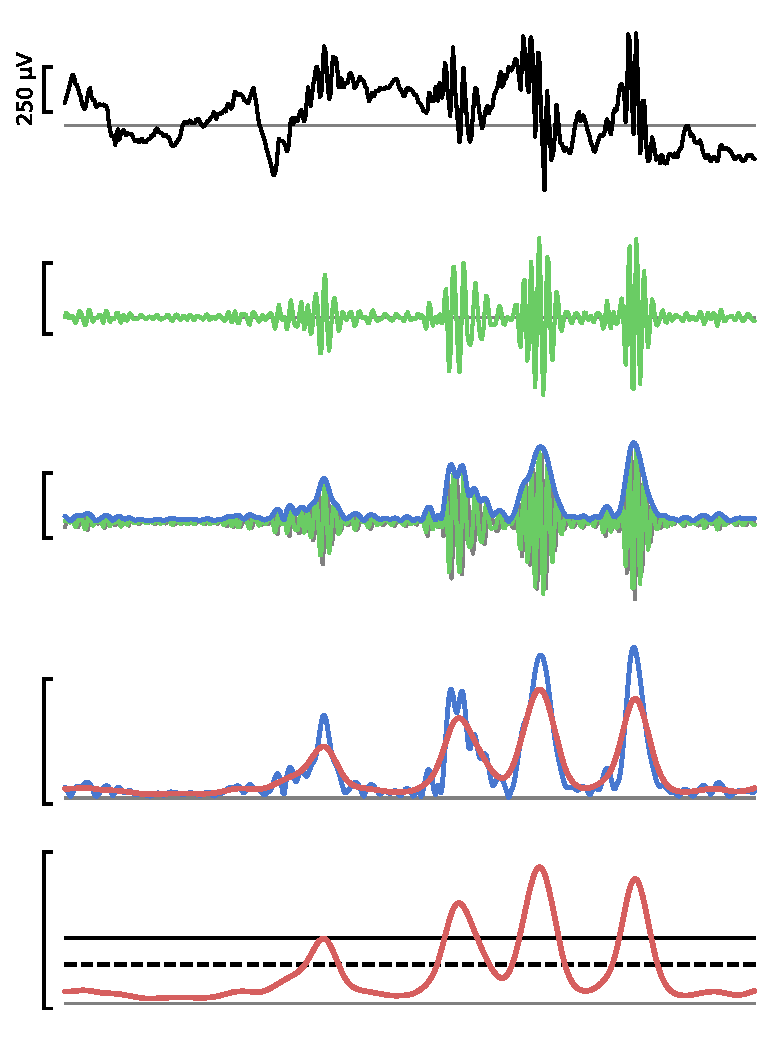
\includegraphics{figures/offline-SWR-detection}
\captionn{Steps for automated, offline SWR labelling}{}
\end{figure}

% standardised data
